\documentclass[11pt,a4paper]{report}
\usepackage[latin1]{inputenc}
\usepackage[spanish]{babel}
\usepackage{amsmath}
\usepackage{amsfonts}
\usepackage{amssymb}
\usepackage{graphicx}
\usepackage{hyperref}
\usepackage[left=2cm,right=2cm,top=2cm,bottom=2cm]{geometry}

%%%%%%%%%%%%%%%%%%%% CONFIG COLORES LINEA COMANDOS
\usepackage{color}
\definecolor{gray97}{gray}{.97}
\definecolor{gray75}{gray}{.75}
\definecolor{gray45}{gray}{.45}

\usepackage{listings}
\lstset{ frame=Ltb,
     framerule=0pt,
     aboveskip=0.5cm,
     framextopmargin=3pt,
     framexbottommargin=3pt,
     framexleftmargin=0.4cm,
     framesep=0pt,
     rulesep=.4pt,
     backgroundcolor=\color{gray97},
     rulesepcolor=\color{black},
     %
     stringstyle=\ttfamily,
     showstringspaces = false,
     basicstyle=\small\ttfamily,
     commentstyle=\color{gray45},
     keywordstyle=\bfseries,
     %
     numbers=left,
     numbersep=15pt,
     numberstyle=\tiny,
     numberfirstline = false,
     breaklines=true,
   }

% minimizar fragmentado de listados
\lstnewenvironment{listing}[1][]
   {\lstset{#1}\pagebreak[0]}{\pagebreak[0]}
 
\lstdefinestyle{consola}
   {basicstyle=\scriptsize\bf\ttfamily,
    backgroundcolor=\color{gray75},
   }
 
\lstdefinestyle{C}
   {language=C,
   }

%%%%%%%%%%%%%%%%%%%%%%


\author{Miguel Ignacio S�nchez }
\title{\textbf{Anexos PROYECTO TURING}}


\begin{document}
%\maketitle

\chapter*{Anexo I: Comandos Git para manejar repositorios.}
A continuaci�n vamos a listar los comando que utilizamos en el terminal de Ubuntu para manejar los repositorios de nuestro proyecto.

 \begin{itemize}
 \item \textbf{status}: Para listar los ficheros que hemos modificado y cuales est�n pendientes de commit o add.
 \item \textbf{add}: Para a�adir ficheros nuevos al repositorio. (Ej: git add sample.cpp).
 \item \textbf{rm}: Para borrar ficheros del repositorio remoto. (Ej: git rm sample.cpp).
 \item \textbf{commit}: Para indicarle al repositorio que es lo nuevo que queremos subir o guardar. (Ej. git commit -m $"some message"$).
 \item \textbf{push}: Se hace para empujar o subir nuestros cambios al repositorio remoto. Tenemos que indicarle a que rama queremos subir nuestro repositorio. (Ej. git push origin master).
 \item \textbf{pull}: Coger descargar los cambios del repositorio remoto.(Ej. git pull).
 \item \textbf{diff}: Para pre-visualizar cambios entre el repositorio y nuestra copia local.(Ej. git diff).
 \item \textbf{init}: Para crear nuevos repositorios locales. (Ej. git init).
 \item \textbf{clone}: Para hacer clonar repositorios. se pueden hacer copias de nuestro repositorio local en otra carpeta local (Ej. git clone /path...). Tambi�n se pueden clonar repositorios remotos (Ej. git clone username@host:path/to/repository).
 \item \textbf{help}: Para obtener ayuda sobre los comandos de git. (Ej: git help).
 \end{itemize}

\chapter*{Anexo II: ROS crear workspace y paquetes.}
\section{Workspace}
Para crear el workspace, tenemos que seguir los siguientes pasos:

\begin{listing}[style=consola, numbers=none]
 \$ mkdir -p ~/catkin_ws/src*)
 \$ cd ~/catkin_ws/
 \$ catkin_make 
\end{listing}

Para cargar nuestro workspace y ponerlo al principio del path de ROS, con lo que conseguimos que ante dos paquetes con el mismo nombre se coja la que primero esta en el path).

\begin{listing}[style=consola, numbers=none]
source devel/setup.bash
\end{listing}

Comprobamos ROS PATH con:
 
\begin{listing}[style=consola, numbers=none]
echo \$ROS_PACKAGE_PATH
\end{listing}

\section{Python package}
Para crear paquetes no importa el lenguaje que estamos utilizando, solo tenemos que tener en cuenta que debemos de a�adirlo a las dependencias, el modelo para crear paquetes es el siguiente:

\begin{listing}[style=consola, numbers=none]
# This is an example, do not try to run this
# catkin_create_pkg <package_name> [depend1] [depend2] [depend3]
\end{listing}

A continuaci�n mostramos un ejemplo.
\begin{listing}[style=consola, numbers=none]
\$ catkin_create_pkg beginner_tutorials std_msgs rospy roscpp
\end{listing}



\chapter*{Anexo III: Comandos utilies}

En este anexo vamos a ir listando los diferentes comandos que nos pueden ser utilies para Ubuntu, ROS, etc.

\begin{itemize}

\item Buscas paquetes disponibles en ROS: 
\begin{listing}[style=consola, numbers=none]
 sudo apt-cache search ros-indigo | grep opencv
\end{listing}

\end{itemize} 


\chapter*{Anexo IV: Paquetes necesarios }

Paquetes necesarios para abrir simulador chefbot:
\begin{itemize}
 \item sudo apt-get install ros-indigo-turtlebot-description
 \item sudo apt-get install ros-indigo-turtlebot-bringup
\end{itemize}


\chapter*{Anexo V: Configurar Qtcreator}
%Capitulo a modificar, utilizando el pliguin de ROS para qutcreator.%
% https://ros-qtc-plugin.readthedocs.io/en/latest/ %
Con este anexo quiero dejar claro como tengo que configurar Qtcreator para ide de desarrollo para ROS.  

	\begin{enumerate}
	\item Tenemos que abrir Qtcreator desde terminal, por que autom�ticamente carga el fichero $~/.bashrc$ el cual es el encargado de configurar el workspace 		de ROS.
	\item Una vez abierto el IDE de programaci�n Qtcreator los siguiente es abrir el proyecto CMakelist de orden mas superior, es decir, 								$~/catkin_ws/src/CMakelist$. Este es el truco, este enlaza directamente con toda la instalaci�n de ROS.
	\item Despu�s de abrir el proyecto, configuramos el directorio build a \url{$catkin_ws/build/$} 
	\item en los argumentos de Cmake ponemos: $-DCMAKE_INSTALL_PREFIX=../install$ \\
	$-DCATKIN_DEVEL_PREFIX=../devel$ 
	\item Hacemos click derecho sobre el directorio del proyecto y hacemos run CMake.  
	\end{enumerate}

Probamos $https://answers.ros.org/question/91516/qt-creator-281-ros-and-catkin-problems/$

\chapter*{Anexo VI: Tiva C Launchpad}

A continuaci�n voy a anotar informaci�n importante sobre la placa, 

\section{Pin Maps}

\begin{figure}[h!]
		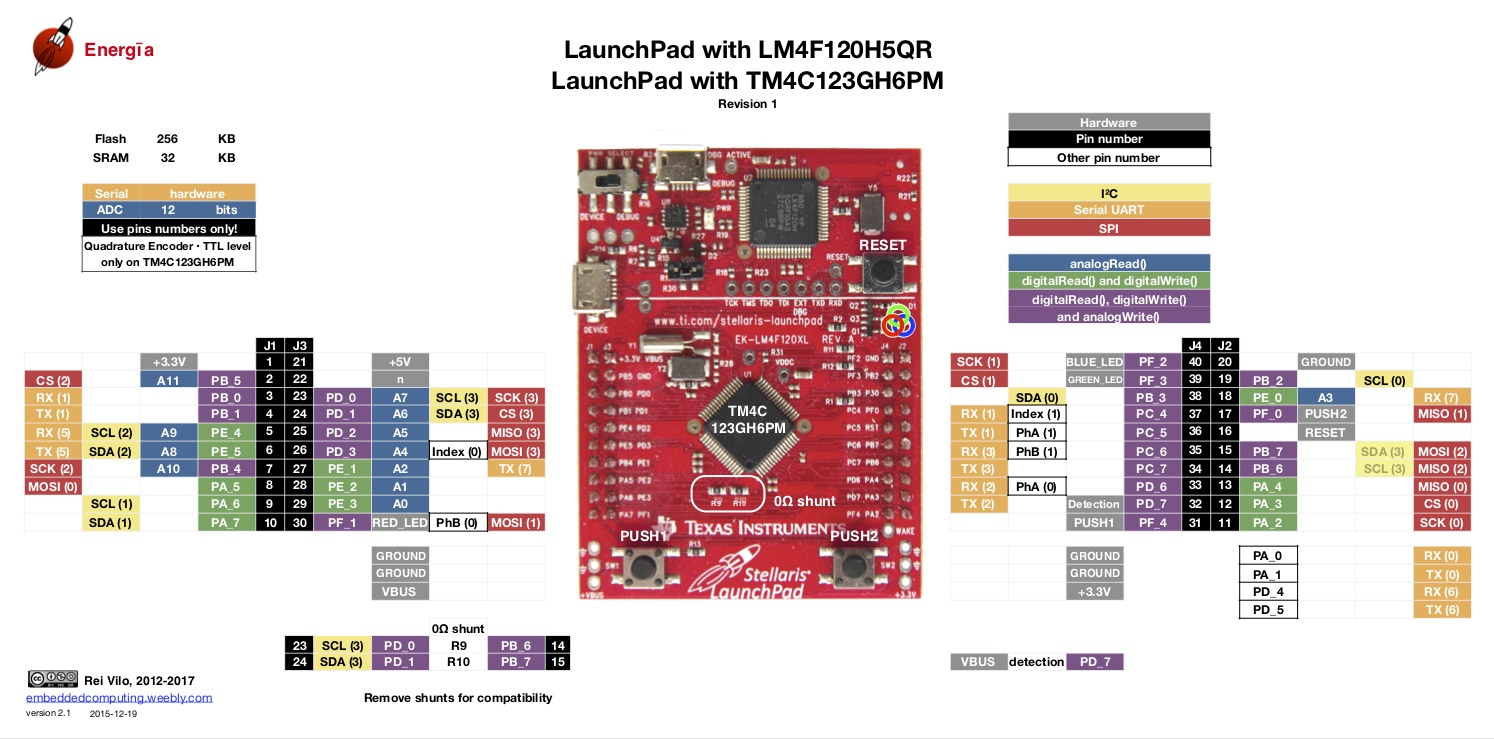
\includegraphics[scale=0.3]{imagenes/EK-TM4C123GXL.jpg}
		\label{fig:5}
		\centering
		\caption{Sensor Ultrasonido HC-SR04}
\end{figure}

\begin{figure}[h!]
		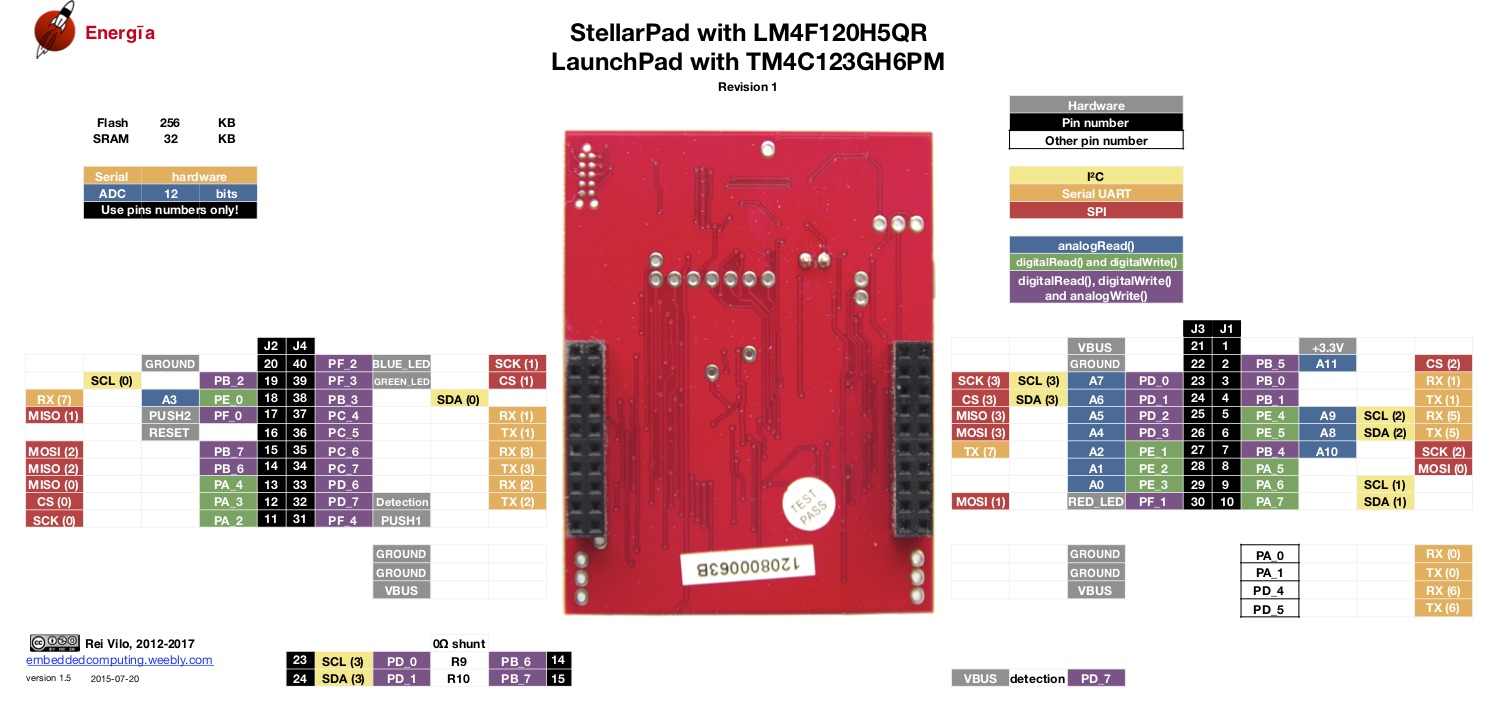
\includegraphics[scale=0.3]{imagenes/EK-TM4C123GXL-BACK.jpg}
		\label{fig:5}
		\centering
		\caption{Sensor Ultrasonido HC-SR04}
\end{figure}

\section{Tutoriales}



\end{document}